%-----------------------------------------------------------------------------------------------------------------------------------------------------------------------------------------------
% Resultados/Discussões: 
% Aqui se mostra o que o trabalho permitiu produzir, e às vezes o que pode ser comparado com outros trabalhos
% Aqui ficam claras se as propostas do trabalho são relevantes ou não, pois devem permitir a discussão do trabalho;
% Deve-se responder: Os resultados estão claros em bom número (nem muito nem pouco) que permitam avaliar realmente a proposta e o que foi produzido.
\chapter{Resultados}
\label{Resultados}

Os resultados apresentados neste capítulo estão divididos em duas partes. Os resultados da seção \ref{resultsGUI} estão inteiramente relacionados as funções fundamentais presentes na interface gráfica desenvolvida. Já na seção \ref{resultsComparison}, tem-se presente os resultados que apresentam os dados obtidos através dos testes de desempenho dos métodos de \textit{Stereo Matching} nas plataformas utilizadas.

%-----------------------------------------------------------------------------------------------------------------------------------------------------------------------------------------------
\section{Interface Gráfica - \textit{StereoVisionGUI}}
\label{resultsGUI}

Nesta seção, o software desenvolvido apresenta uma interface gráfica (GUI -- \textit{Graphical User Interface}) amigável, a qual facilita a visualização das imagens da câmera estéreo, 
dos mapas de disparidades, da reconstrução tridimensional e do método de processamento de imagens desenvolvido. Atualmente, o software conta com três métodos para encontrar correspondências 
estéreo (BM, SGBM e BMGPU) e com 8 opções das quais 6 delas são destinadas a visualização das seguintes perspectivas:

\begin{enumerate}
  \item Imagens retificadas das câmeras esquerda e direita
  \item Mapa de disparidades em Escala de Cinza e RGB
  \item Mapa tridimensional do ambiente reconstruído em Escala de Cinza e RGB
  \item Imagem da Câmera Esquerda com o indicador de objeto rastreado e Imagem binária resultante da limiarização por distância.
  \item Imagem resultante do processo de detecção de movimentos e Imagem resultante do processo de detecção de movimentos limiarizada por distância. 
  \item Imagem resultante da adição da imagem à direita com a Imagem da Câmera Esquerda e Imagem resultante do processo de realce das bordas dos objetos em movimento próximos ao veículo.
\end{enumerate} 

O botão \textit{Show Left/Right} seleciona a opção na qual a interface gráfica permite a visualização simultânea das imagens retificadas de ambas câmera. A figura \ref{gui_showleftright_view} 
ilustra o comportamento do software quando essa opção é selecionada. 

O botão \textit{Show Disparity Map} seleciona a opção na qual a interface gráfica permite a visualização simultânea dos mapas de disparidade em escala de cinza e RGB. A figura 
\ref{gui_showdisparitymap_view} ilustra o comportamento do software quando essa opção é selecionada. 

O botão \textit{Show 3D Reconstruction} seleciona a opção na qual a interface gráfica permite a visualização simultânea dos mapas tridimensionais do ambiente reconstruído em escala de cinza e 
RGB. A figura \ref{gui_show3dreconstruction_view} ilustra o comportamento do software quando essa opção é selecionada. 

O botão \textit{Show Tracking Object View} seleciona a opção na qual a interface gráfica permite a visualização simultânea da imagem da câmera Esquerda com o indicador de objeto rastreado e 
imagem binária resultante da limiarização por distância. A figura \ref{gui_show_tracking_object_view} ilustra o comportamento do software quando essa opção é selecionada. 

O botão \textit{Show DiffImage} seleciona a opção na qual a interface gráfica permite a visualização simultânea da imagem resultante do processo de detecção de movimentos e imagem resultante do 
processo de detecção de movimentos limiarizada por distância. A figura \ref{gui_showdiffimage_view} ilustra o comportamento do software quando essa opção é selecionada. 

O botão \textit{Show Warning Edges} seleciona a opção na qual a interface gráfica permite a visualização simultânea da imagem resultante da adição da imagem à direita com a imagem da câmera esquerda e imagem resultante do processo de realce das bordas dos objetos em movimento próximos ao veículo. A figura \ref{gui_showwarningedges_view} ilustra o comportamento do software quando essa opção é selecionada. 


\begin{figure}[H]
 	\centering
 	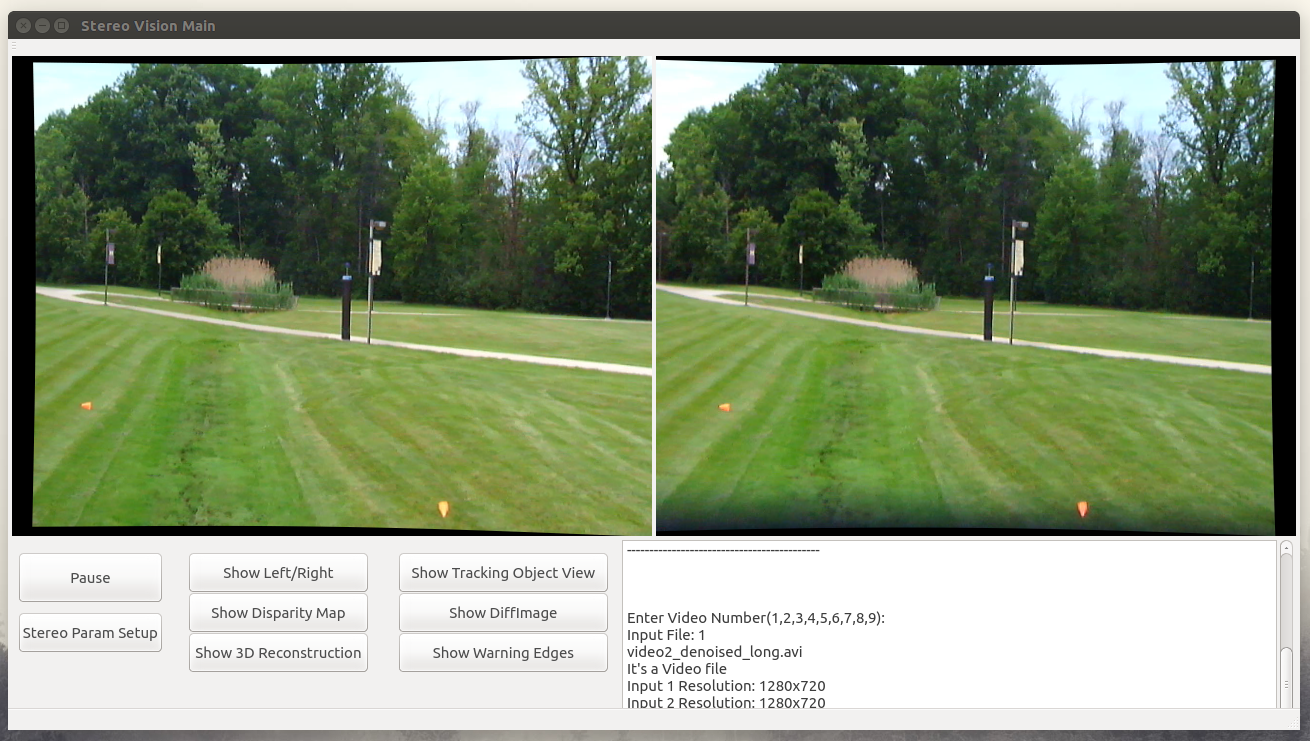
\includegraphics[scale=0.35]{./Resources/gui_showleftright_view.png}
 	\caption{Interface Gráfica - Visualização simultânea dos quadros das câmeras esquerda e direita}
 	\label{gui_showleftright_view}
\end{figure}


\begin{figure}[H]
 	\centering
 	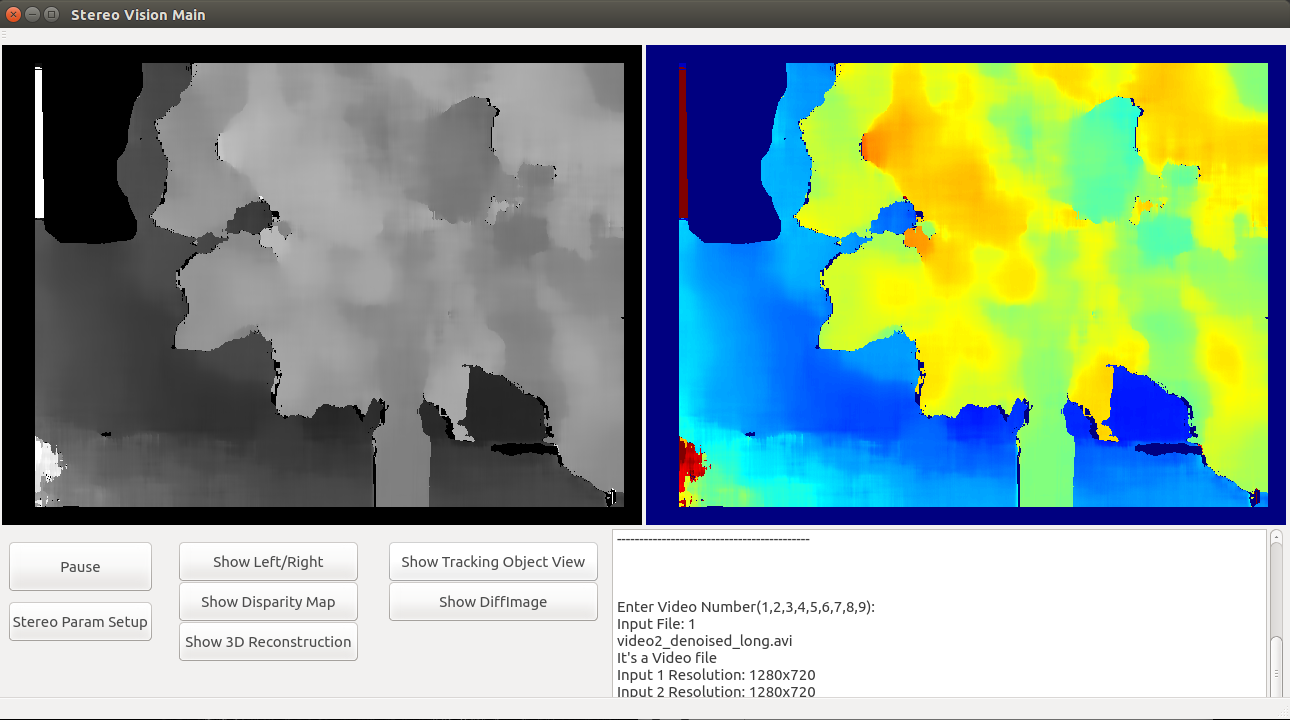
\includegraphics[scale=0.35]{./Resources/gui_showdisparitymap_view.png}
 	\caption{Interface Gráfica - Visualização dos Mapa de disparidades em Escala de Cinza e RGB}
 	\label{gui_showdisparitymap_view}
\end{figure}


\begin{figure}[H]
 	\centering
 	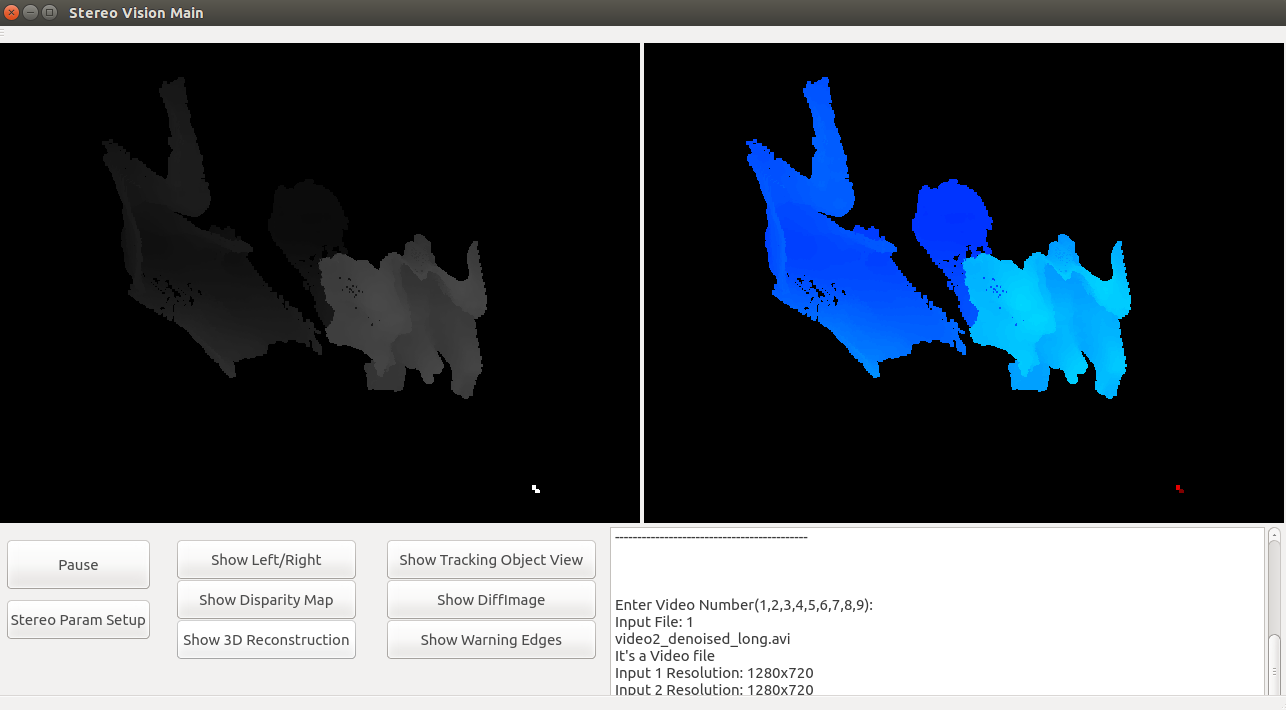
\includegraphics[scale=0.35]{./Resources/gui_show3dreconstruction_view.png}
 	\caption{Interface Gráfica - Visualização dos Mapa de disparidades em Escala de Cinza e RGB}
 	\label{gui_show3dreconstruction_view}
\end{figure}


\begin{figure}[H]
 	\centering
 	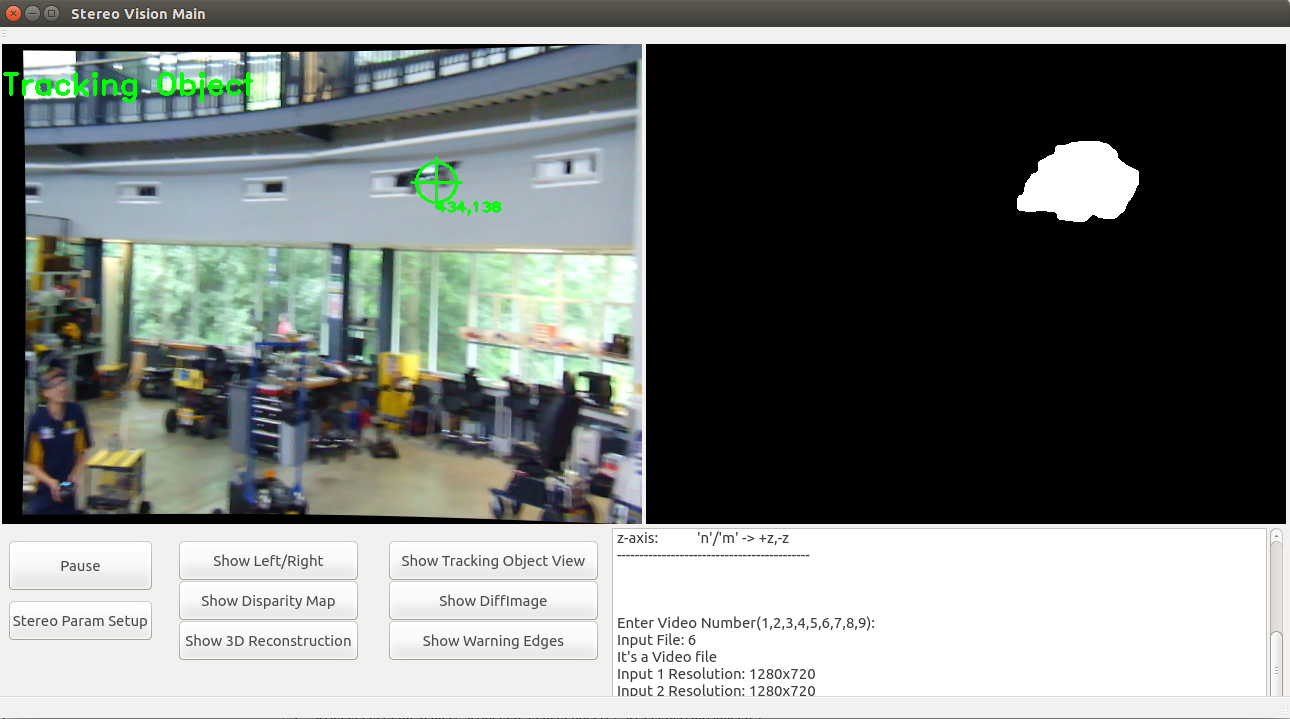
\includegraphics[scale=0.35]{./Resources/gui_show_tracking_object_view.png}
 	\caption{Interface Gráfica - Visualização da Imagem da Câmera Esquerda com o indicador de objeto rastreado e da Imagem binária resultante da limiarização por distância}
 	\label{gui_show_tracking_object_view}
\end{figure}


\begin{figure}[H]
 	\centering
 	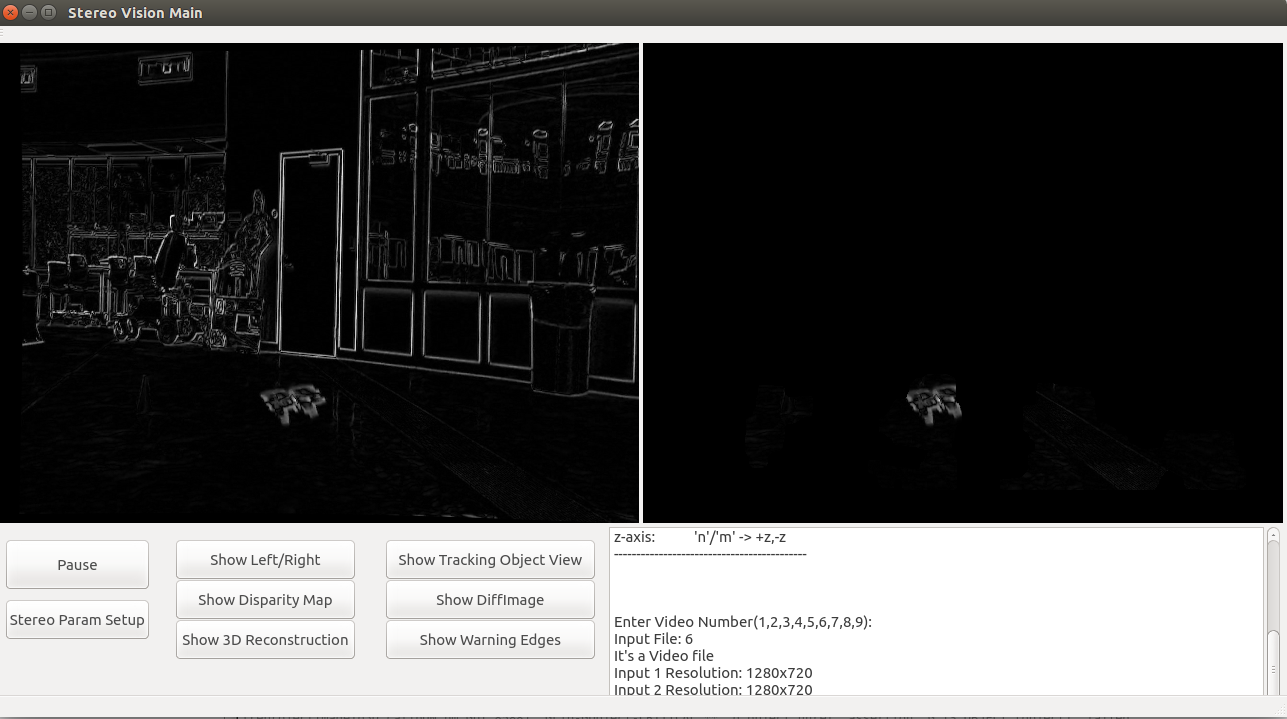
\includegraphics[scale=0.35]{./Resources/gui_showdiffimage_view.png}
 	\caption{Interface Gráfica - Visualização da imagem resultante do processo de detecção de movimentos e imagem resultante do processo de detecção de movimentos limiarizada por distância}
 	\label{gui_showdiffimage_view}
\end{figure}


\begin{figure}[H]
 	\centering
 	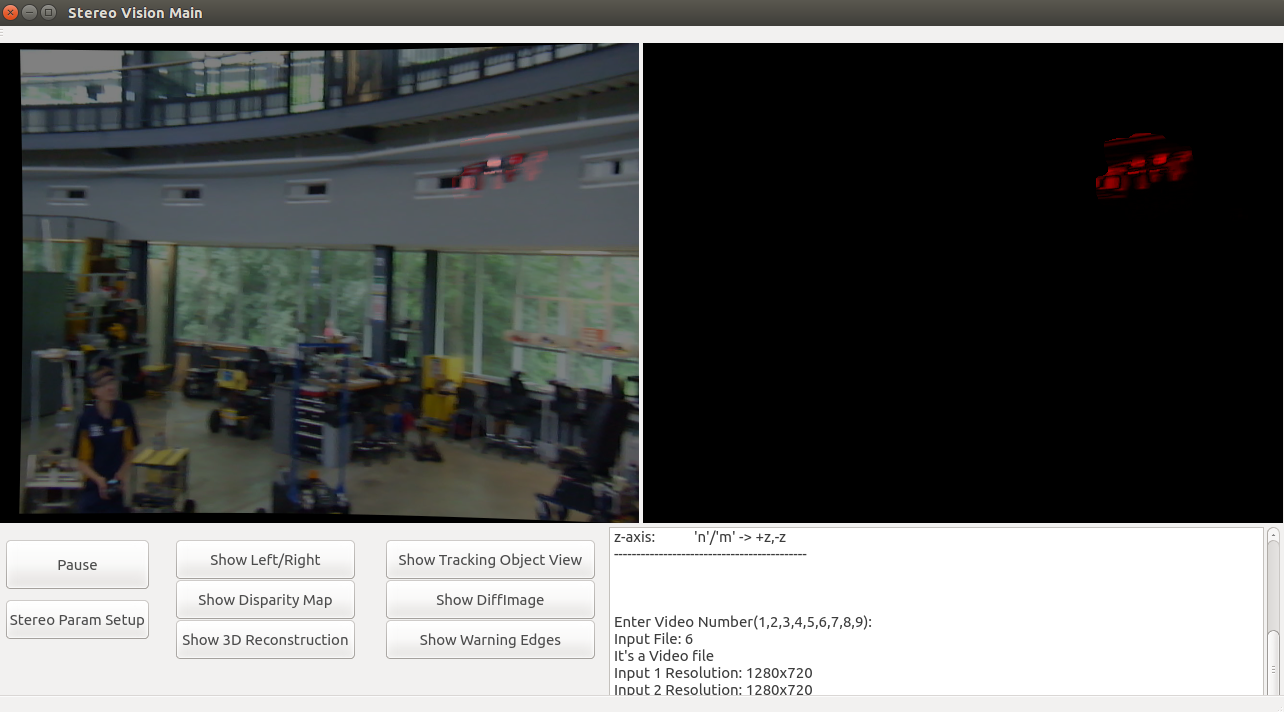
\includegraphics[scale=0.35]{./Resources/gui_showwarningedges_view.png}
 	\caption{Interface Gráfica - Visualização da Imagem resultante da adição da imagem à direita com a Imagem da Câmera Esquerda e Imagem resultante do processo de realce das bordas dos 
 	objetos em movimento próximos ao veículo}
 	\label{gui_showwarningedges_view}
\end{figure}

% TODO: Colocar Novas Imagens com os resultados mais bonitos. Tirar fotos de uma mesma cena comparativamente ao 3 métodos


%-----------------------------------------------------------------------------------------------------------------------------------------------------------------------------------------------
\section{Comparação de Desempenho: Desktop x BBB x Jetson TK1}
\label{resultsComparison}

Nesta seção, estão apresentados os resultados práticos das diferentes implementações dos métodos de visão estéreo nas plataformas abordadas. Os Métodos utilizados foram BM, SGBM e BMGPU para a comparação das plataformas. O método BMGPU mostrou-se o de melhor performance, visto que é o que requisita menor processamento dentre os outros métodos mais conhecidos (SGBM, BP, CSBP, AD Census, ...) além de ser acelerado em hardware. A tabela \ref{resultsCPUGPU} abaixo, apresenta o resultado de desempenhos obtidos nas plataformas, apresentando comparativamente seu desempenho quando o processado utilizando CPU ou GPU/NEON (Caso da BBB). Com relação à configuração utilizada para a realização dos teste, utilizou-se uma resolução de 640x480, um tamanho média da janela usada para combinar blocos de pixels (\textit{SADWindowSize}) de 15 e um tamanho da gama de disparidades (\textit{NumberOfDisparities}) igual à 16, como pode ser observado na tabela \ref{teste_values}. O critério de escolha desses valores foi dado pelo balanço entre performance e qualidade do mapa de disparidades gerado, isto é, um mapa que fosse confiável e permitisse as corretas correspondências do mapa de disparidades.

O gráfico da figura \ref{grafico_desempenho} apresenta o comparativo entre o desempenho de cada plataforma para os métodos estéreo BM, SGBM e BMGPU. O resultado da BBB para o método BM é muito inferior aos resultados obtidos nas demais plataformas. O teste para o método SGBM foi abortado, visto que naturalmente este método é um algoritmo mais complexo que o BM. Decorrente a isso, espera-se que sua performance seja inferior à um FPS. Segundo o manual da BBB, o processador ARM Cortex A8 apresenta suporte ao NEON™, o qual é um acelerador de ponto flutuante que utiliza instruções SIMD (\textit{Single instruction, Multiple Data}) para a aceleração de algoritmos de multimídia e processamento de sinais \cite{ARMNEON}. Os testes dos métodos estéreo na BBB utilizando essa tecnologia também não foram executados, pois sua implementação tomaria um tempo considerável e provavelmente não apresentaria um resultado expressivo. 

\begin{table}[]
\centering
\caption{Configuração utilizada para Avaliação de Performance}
\label{teste_values}
\begin{tabular}{|c|c|}
\hline
                    & Configuração \\ \hline
Resolução           & 640x480      \\ \hline
SADWindowSize       & 15           \\ \hline
NumberOfDisparities & 16           \\ \hline
\end{tabular}
\end{table}

\begin{table}[]
\centering
\caption{Desempenho atingido por cada plataforma dos Métodos Utilizados}
\label{resultsCPUGPU}
\begin{tabular}{|c|c|c|c|}
\hline
Quadros por Segundo (FPS)       & BM & SGBM & BM\_GPU  \\ \hline
Desktop   & 28 & 12   & 30       \\ \hline
BBB       & 1  & -    & -        \\ \hline
Jetson TK1 & 6  & 2    & 7$\sim$8 \\ \hline
\end{tabular}
\end{table}

\begin{figure}[H]
 	\centering
 	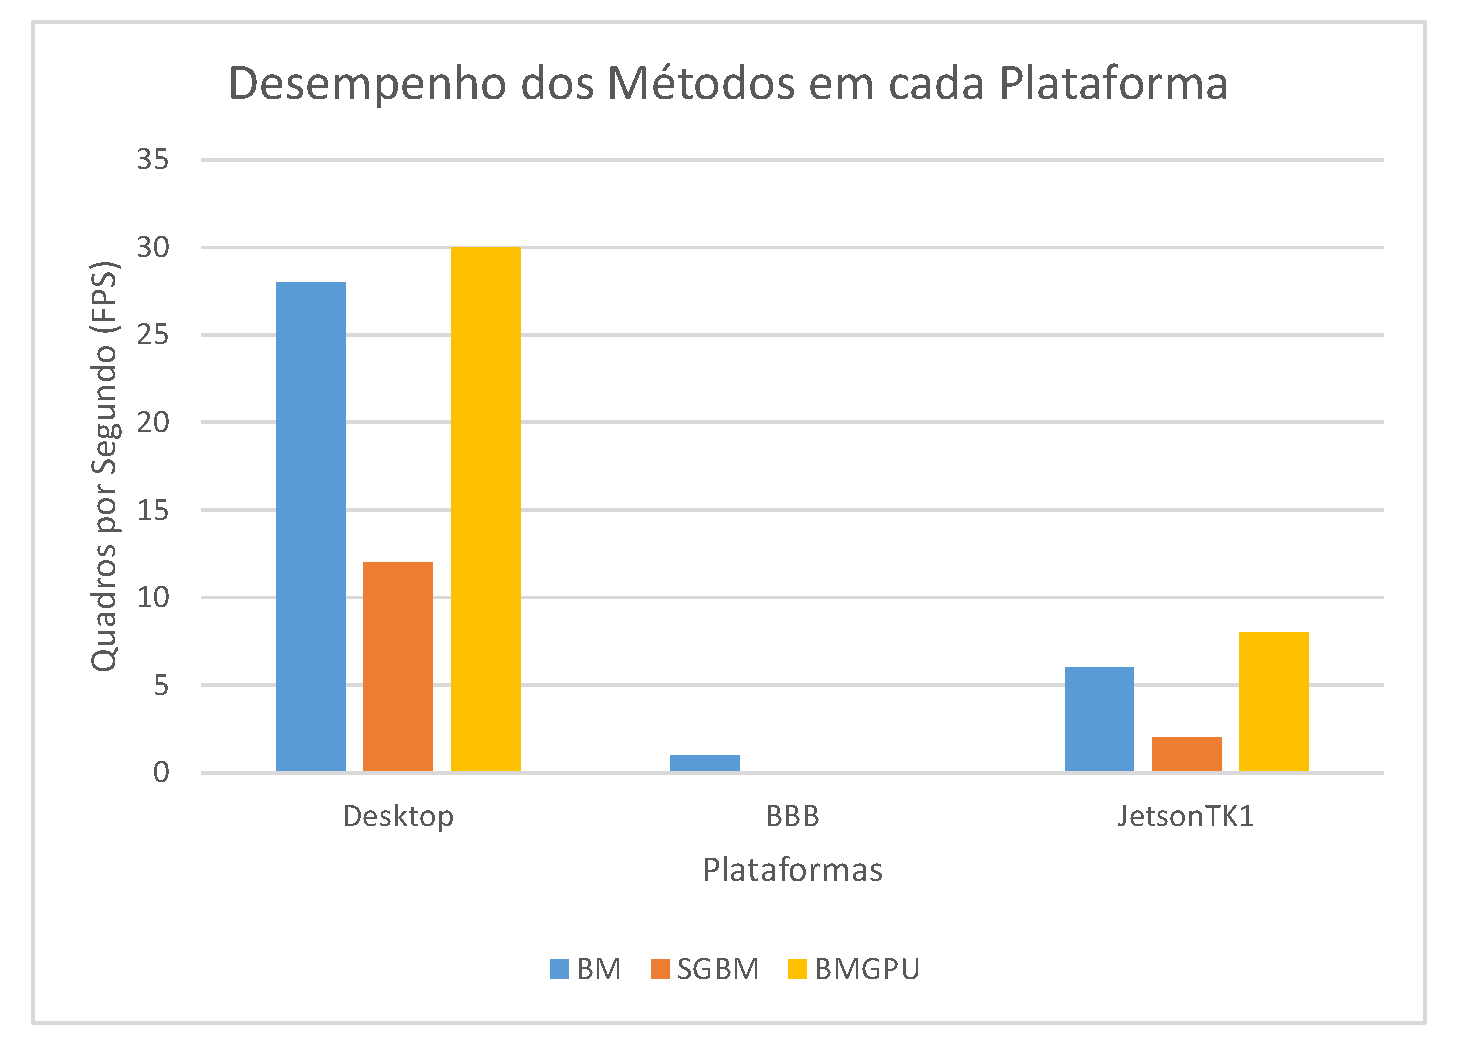
\includegraphics[scale=0.5]{./Resources/grafico_desempenho.pdf}
 	\caption{Gráfico - Comparação de Desempenho dos Métodos Estéreo para cada plataforma.}
 	\label{grafico_desempenho}
\end{figure}

% TODO: Descrever cada Item
%-----------------------------------------------------------------------------------------------------------------------------------------------------------------------------------------------
\subsection{Desktop}
\subsubsection{CPU}

Primeiramente, as rotinas para execução em CPU foram implementadas no \textit{Desktop} e só então foram adaptadas para as plataformas embarcadas. Os valores de desempenho obtidos foram usados como referência para a comparação com os resultados acelerados por GPU e com as plataformas embarcadas. Como esperado, o SGBM mostrou-se mais lento que o BM, isso deve-se ao fato do algoritmo ser mais complexo por conta da análise global realizada (Mais detalhes em \ref{stereo_methods}). 

\subsubsection{GPU}

Como previsto, o desempenho do método BM acelerado em GPU é superior ao executado em CPU. Consequentemente, este resultado motivou a implementação do mesmo na plataforma \textit{Jetson TK1}, visto que sua implementação é bastante similar a em Desktop por conta de possuírem a mesma arquitetura de GPU (Kepler).  

%-----------------------------------------------------------------------------------------------------------------------------------------------------------------------------------------------
\subsection{BeagleBone Black(BBB)}
\subsubsection{CPU}

O resultado obtido para o método BM desmotivou qualquer outra implementação nesta plataforma. Dificilmente algum outro recurso de aceleração apresentaria um resultado que realizasse o processamento de imagens necessários com resposta em tempo real. permitisse a utilização de algoritmos de processamento de imagens para a resposta de 

\subsubsection{NEON}


%-----------------------------------------------------------------------------------------------------------------------------------------------------------------------------------------------
\subsection{Jetson TK1}
\subsubsection{CPU}
\subsubsection{GPU}